\section{The input-length variable and the canvas Pareto}
\label{app:input_canvas}

\subsection{Input length: the second variable}

Each denoising step re-attends the full prompt, so prefill is paid $K$
times. DG's prefill slope is \inputSlopeRatio$\times$
steeper than the autoregressive model's. At longer inputs the diffusion
base rises faster and pushes $L^{*}$ upward
(Figure~\ref{fig:input}).

\begin{figure}[ht!]
\centering
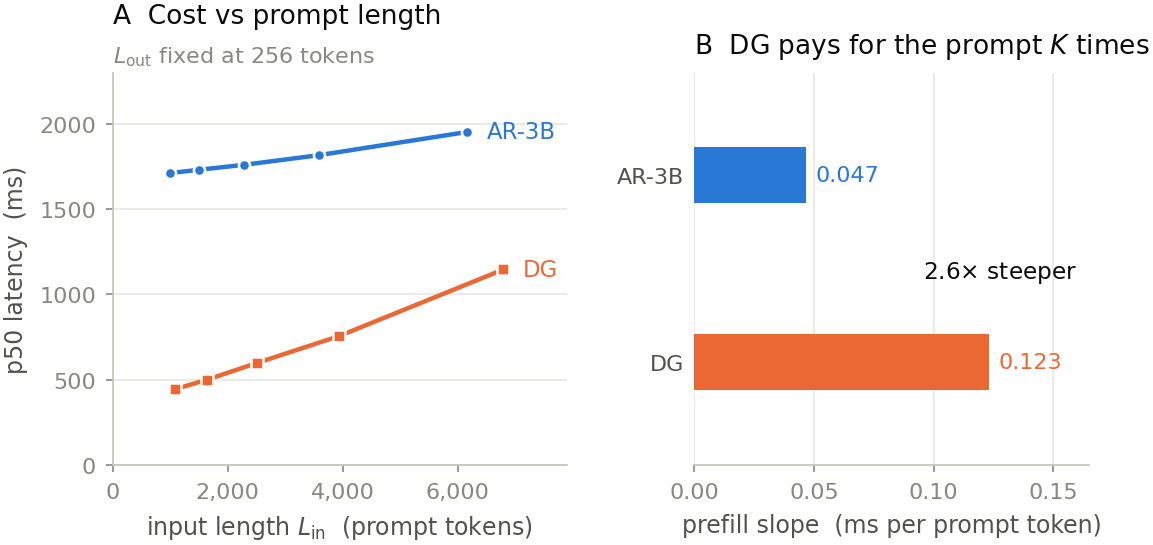
\includegraphics[width=\linewidth]{figures/fig3_input_sweep.png}
\caption{Input-length sweep at fixed $L_{\mathrm{out}}{=}\canvasLength$
(BGL, $n{=}100$; AR arm is dense AR-3B). The prompt is lengthened by
repeating the schema block, so the task is unchanged.}
\label{fig:input}
\end{figure}

\subsection{A free Pareto improvement at canvas $= 128$}

At canvas $=128$ the base falls to \canvasOneTwentyEightBase\,ms
($-2.0\%$) \emph{and} 9-field F1 rises to
\canvasOneTwentyEightFone{}, an improvement on both axes
simultaneously. At canvas $=64$ the base rises $48\%$ because the
per-canvas fixed overhead is paid twice as often; that setting is not
viable. Block size, not denoising schedule, is the interesting design
variable. Canvas $=128$ barely moves the crossover, $L^{*}$ falls
from $48$ to $46$ tokens, because the base drops only $2\%$, but
canvas $=64$ pushes it to $L^{*}\approx73$, since $L^{*}$ scales with
the base and that base is $48\%$ higher. Shrinking the canvas doesn't
shrink the prefill it must re-attend, so a smaller canvas buys
finer-grained output at the cost of paying the fixed overhead more
often.

\subsection{Joint canvas$\times$K sweep confirms canvas $= 128$ is
Pareto-optimal}

A full $4\times5$ grid (canvas $\in \{64,128,256,512\}$, $K \in
\{2,4,8,16,32\}$, $n{=}200$ per cell) confirms the single-knob finding
holds across all $K$ values, not just $K{=}8$. The Pareto frontier
contains six cells; the paper's current operating point (canvas$=256$,
$K{=}8$: p50$=$376\,ms, F1$=$0.853) is \emph{dominated} by
(canvas$=128$, $K{=}8$: p50$=$368\,ms, F1$=$0.864), which is faster
and higher quality simultaneously. The $K$ knee also shifts left at
smaller canvas: at canvas$=128$, $K{=}8$ is near saturation
(F1$=$0.864), while at canvas$=256$ quality keeps improving through
$K{=}32$ (F1$=$0.862). Canvas$=64$ remains non-viable even at $K{=}32$
(F1$=$0.834, below the canvas$=256$ $K{=}8$ baseline). Full data in
\texttt{results/issue114\_joint\_sweep.json}.
